In this chapter we describe the design of convolutional neural network which is able to process thermal images and predict what object they contain.
Workflow that follows will largely be a combination of workflows presented in Figures \ref{ml_workflow} and \ref{micro_workflow}.

We first set concrete objectives, which dictate what exactly we want to accomplish, while keeping in consideration various constraints.
We then explored the dataset provided by the Arribada Initiative, analyzed different class representations and decided, if the dataset is appropriate for accomplishing objectives that we set earlier.
Tools and development environment used in the process are also described.

In image preprocessing phase we imported images and connected them with metadata that was parsed from the excel database.
We analysed the dataset, split it into different sets and applied image correction procedures.
We then decided on few slightly similar CNN architectures with variable hyperparameters and ran a random search algorithm, which found several different models based on accuracy.
In chapter/section TODO ADD REFERNCE we compared models in terms of accuracies and size.
Chosen models were then converted into a C char array format. 

We finish this chapter by going through the same design process again, but this time using tools that Edge Impulse provides. 
In chapter/section TODO ADD REFERENCE we compared on device performance of our modules versus the ones created with Edge Impulse.


\section{ Model objectives}

The accuracy of our early detection system should be equal or similar to the one of human observer, no matter if it is operating in daytime or nighttime.
Although the system will be placed on the paths that are regularly traversed by elephants, they are not only possible objects that can appear on taken thermal images.
Humans and various livestock, such as goats and cows, could also be photographed.
Reporting false positives should be avoided, which means that the system should not incorrectly label a human or a livestock animal as an elephant.
At the same time false negatives also need to be avoided, in these cases an elephant could pass the system undetected.
These kind of mistakes could undermine the community's confidence of the early detection system and defeat the purpose.
This means that besides elephant detection, our focus should be also on correctly classifying humans and livestock, while providing a nature/random class for all other unexpected objects or simply images of nature.

It would be beneficial if thermal camera can take several images of the same object, thus increasing the confidence of computed label of the object.
However this is constrained by the image processing time and camera's field of view.
Thermal camera FLIR Lepton has a horizontal field of view of 57 degrees.
The closer elephant passes by the thermal camera, the quicker he traverses the camera's field of view, thus giving the camera less time for capture.
This problem can be solved by minimizing the execution time of the ML model or by placing the early detection system on position that is far away from expected elephant's path.
As latter option might not be always possible, we should strive to keep the whole image processing time as short as possible.

Finally, as our neural network will be deployed on a microcontroller and not on a computer or a server, we have to keep it lightweight in terms of memory.
Extra model complexity that brings few percents of accuracy does not matter much, if the model is too large to fit on a microcontroller or takes too long to run.


To summarize:
\begin{itemize}
    \item We will create an image classification ML model that will be capable of processing a thermal image and sorting it into one of possible 4 categories: elephant, human, cows and nature/random.
    \item Total image processing time should be as short as possible, we should try to keep it under 2 seconds.
    \item Model should be small enough to fit on a microcontroller of our choice, while still leaving some space for application code. Microcontroller of our choice (STM32F767) has 2 MB of flash memory so model size should be smaller than that.
\end{itemize}


\section{ Exploring the dataset} \label{exploring_dataset}

As mentioned in section \ref{arribada_init} thermal image dataset was provided by Arribada Initiative\cite{wildlabs-winners}\cite{arribada-assam}.
Images in dataset came from two different locations: Assam, India and ZSL Whipsnade Zoo, United Kingdom.

Assam served as a testing ground.
Arribada team positioned two camera traps on two locations that overlook paths commonly used by elephants.
Cameras were built out of Raspberry Pi, PIR sensor, FLIR Lepton 2.5 camera and batteries, all of which were enclosed in a plastic housing.
Insides of the camera and an example of deployed camera can be seen on Figure \ref{assam_camera}.

\begin{figure}[ht]
    \begin{subfigure}{0.5\textwidth}
        \centering
        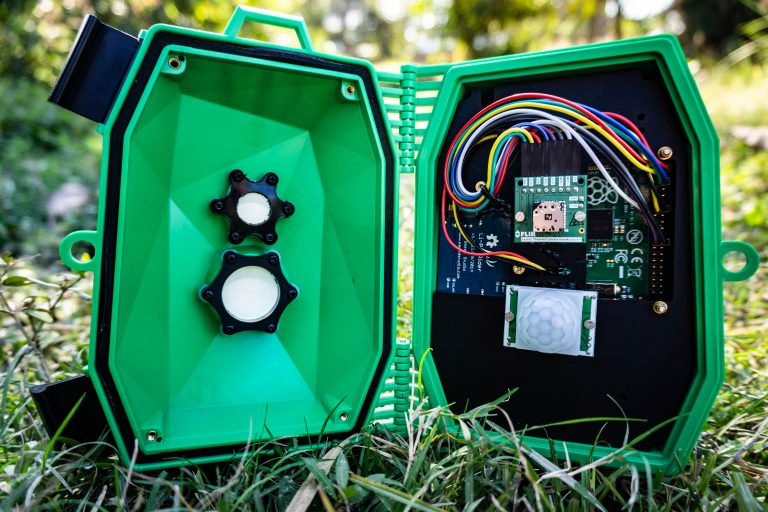
\includegraphics[width=1.0\linewidth, height=5cm]{assam_camera1.jpg} 
    \end{subfigure}
    \begin{subfigure}{0.5\textwidth}
        \centering
        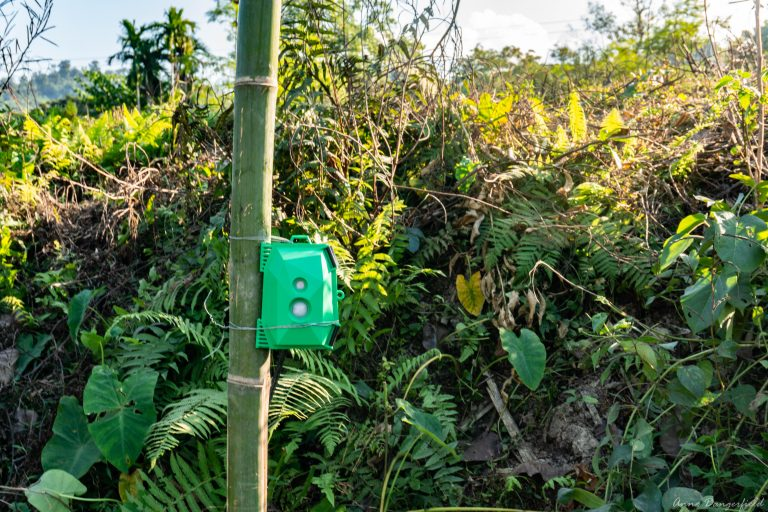
\includegraphics[width=1.0\linewidth, height=5cm]{assam_camera2.jpg}
    \end{subfigure}
    \caption{Camera trap used in Assam, India. Image source: Arribada Initiative \cite{arribada-assam}}
    \label{assam_camera}
\end{figure}

PIR sensor functioned as photo trigger, whenever an object passed in front of it camera made a picture.
This setup provided Arribada with elephant images in real life scenarios, however they could not capture elephants in variety of different conditions, such as different angles and distances.

This was accomplished in ZSL Whipsnade Zoo, where they could take many images of elephants in variety different conditions\cite{dataset_collection}.
PIR sensor trigger approach was dropped in favor of a 5 second time lapse trigger.
Two cameras were used again, however one of them now used FLIR Lepton 3.5 camera with better resolution.

Images of elephants that came from both locations can be seen on Figure \ref{four_elephants}.

\begin{figure}[ht]
    \centering
    \scalebox{.35}{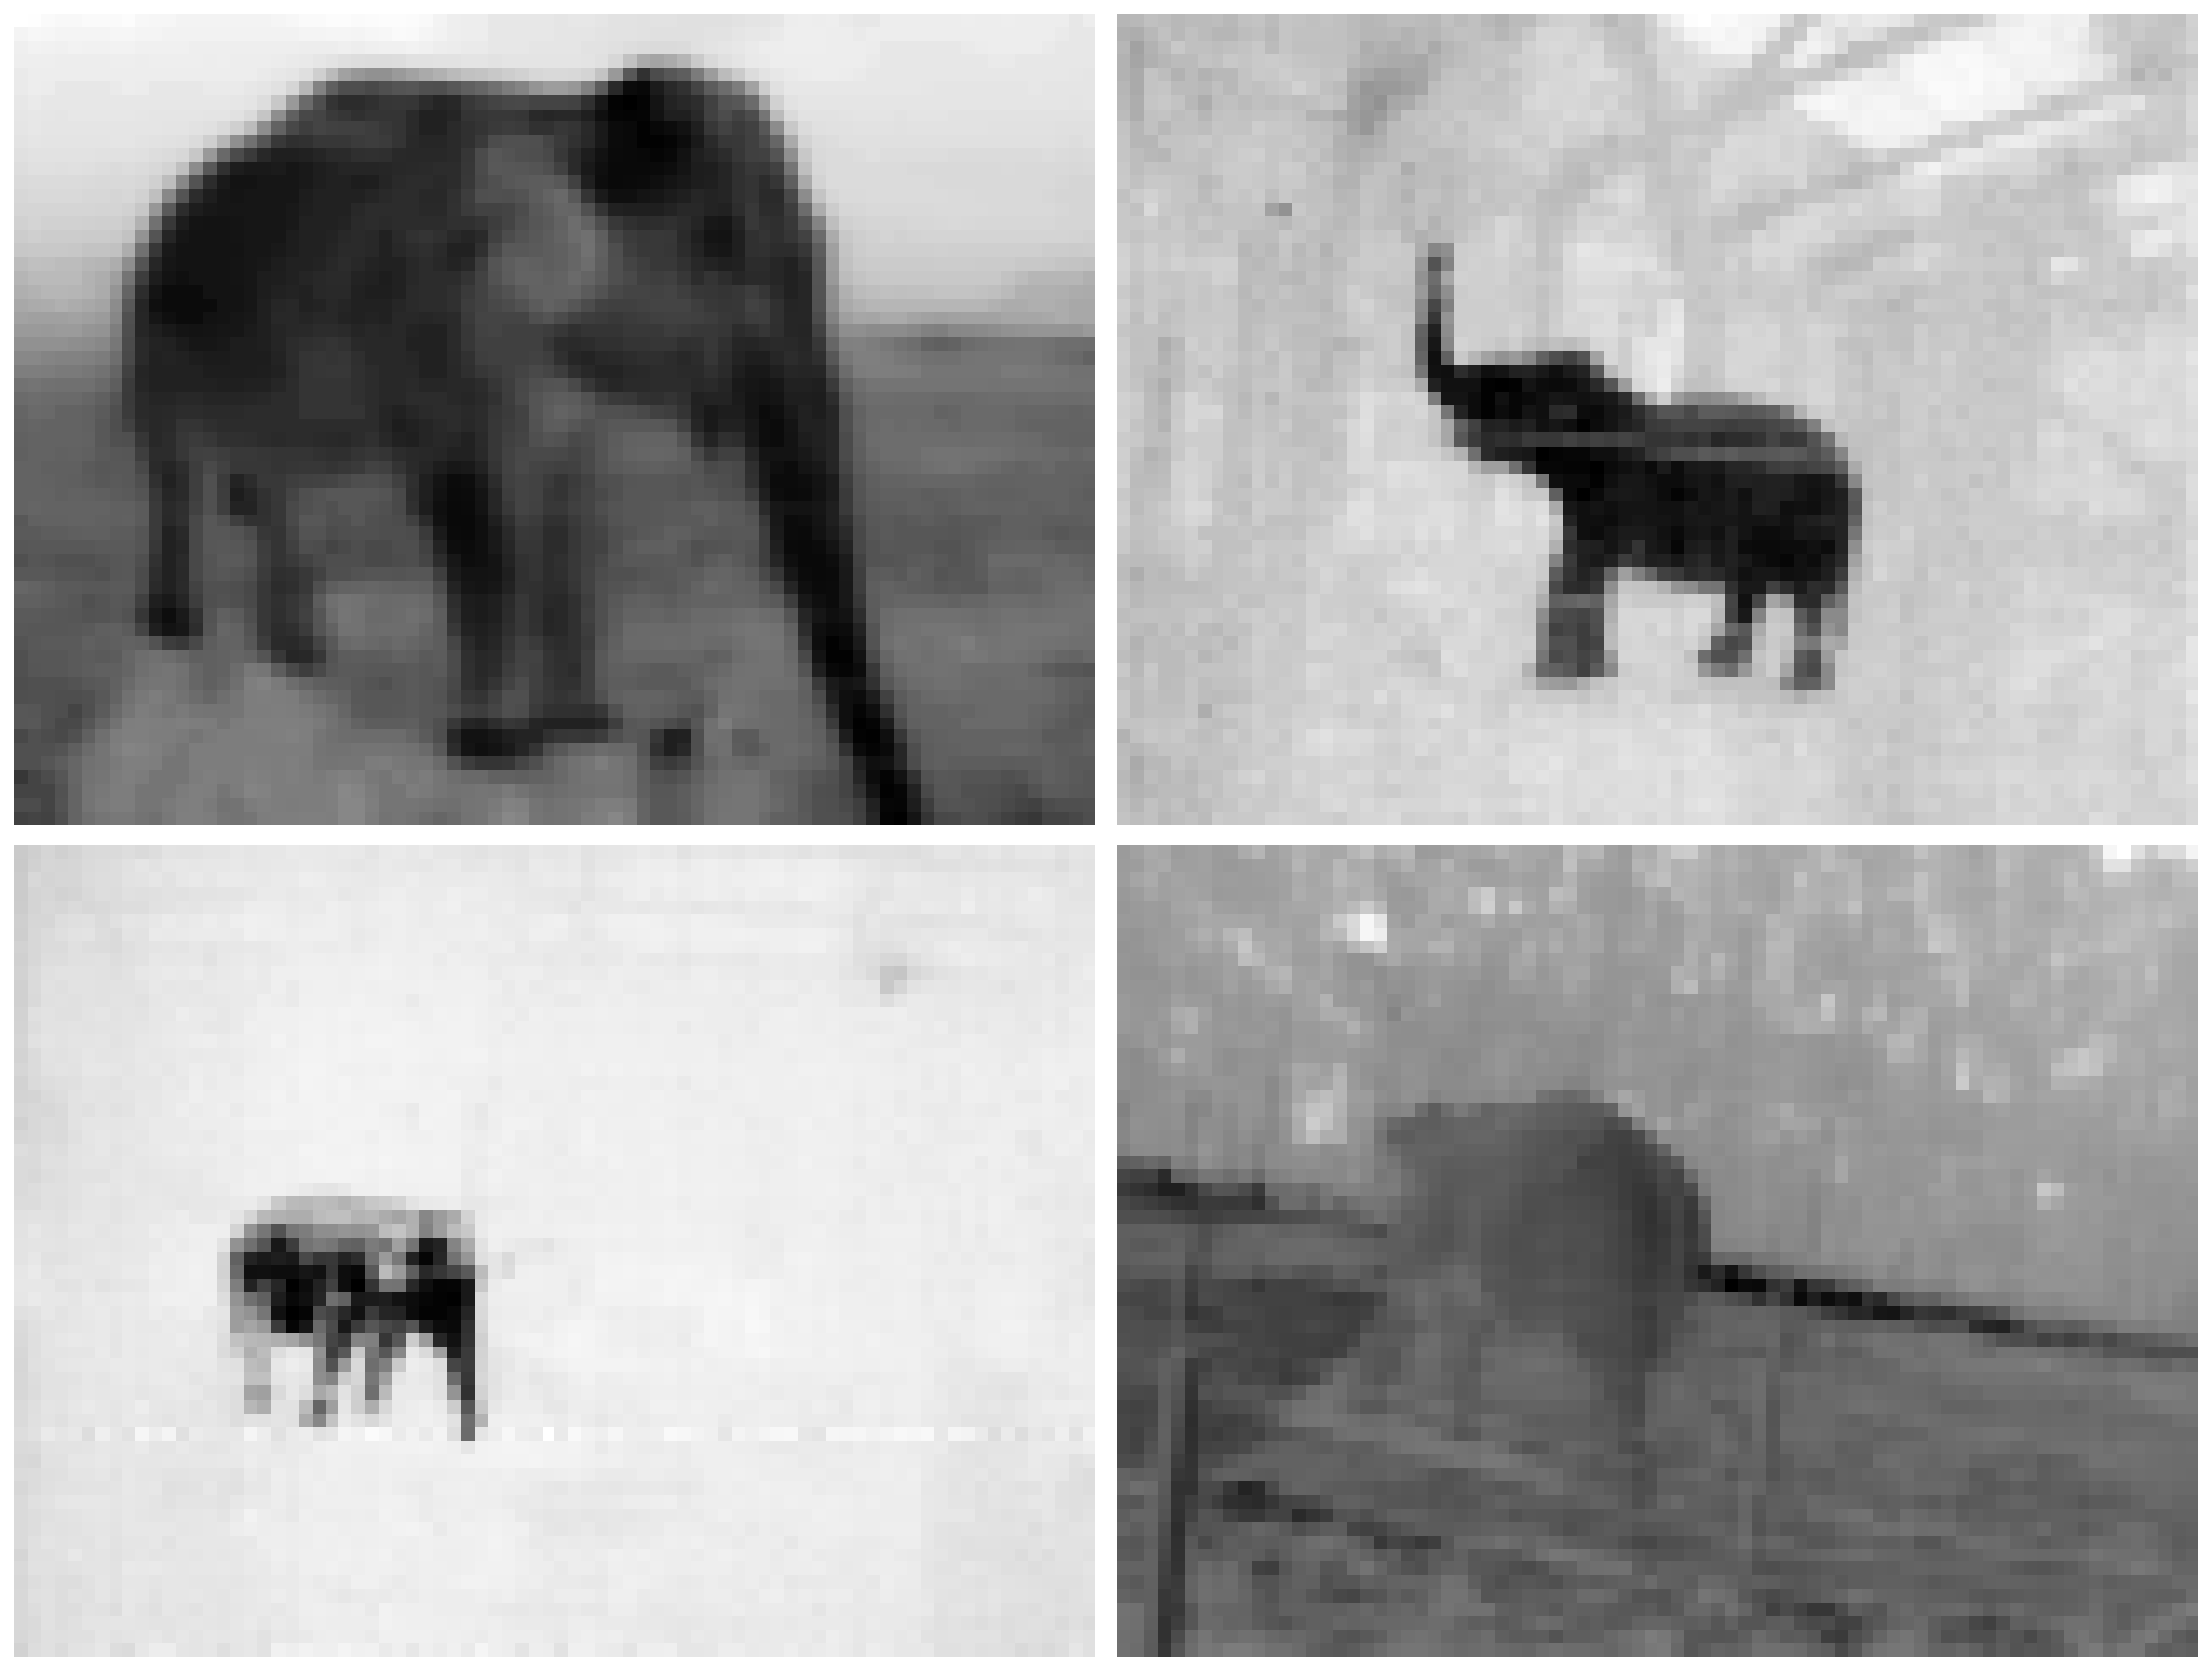
\includegraphics{four_elephants.pdf}}
    \caption{Thermal images of elephants from dataset.}
    \label{four_elephants}
\end{figure}

Thermal image dataset was given to us in form of a Google Drive folder, which we downloaded to our computer.
After examining the folder, we came to several conclusions.

\begin{enumerate}
    \item We saw that the primary focus of Arribada team was to build an object localization model, not an image classification model.
In object localization neural network draws bounding boxes around objects that it recognizes and assigns them labels, while image classification model only labels the image as whole.
Object localization produces a bigger and more complex model than image classification and it is unsuitable for running on a microcontroller.
All major work that was done by Arribada team was contained in one folder where each image had accompanying text file of the same name.
Text files were produced by a DeepLabel software, which is used for preparing images for training object localization models.
Each line in a text file described a location of the bounding box and its label.
This dataset format was not suitable for us, as many images contained more bounding boxes, which would be troublesome to sort into a distinct label.
We later saw that there were few folder with names such as "Human", "Single Elephant", "Multiple Separate Elephants", "Multiple obstructing Elephants", "Cows", "Goats" and so on, which contained sorted images that we could use.
All folders with elephant pictures we merged into one folder, as we did not care if model can differentiate how many elephants are on a taken image, we only wanted to know if there are any elephants on it or not.

    \item We found out that all images were documented in a large Excel database.
For each image there was a row in a database that connected image file name with information where image was taken and with what sensor.
This enabled us to generate a graph seen on Figure \ref{nested_donut1}.
We used a total of 13667 images from thermal image dataset, almost 88 \% of them were made in Whipsnade Zoo, the rest of them were made in Assam.
All images from Assam were made with FLIR Lepton 2.5, while both cameras were used in Whipsnade zoo, however more photos were made with 2.5 version of the thermal camera.

\begin{figure}[ht]
    \centering
    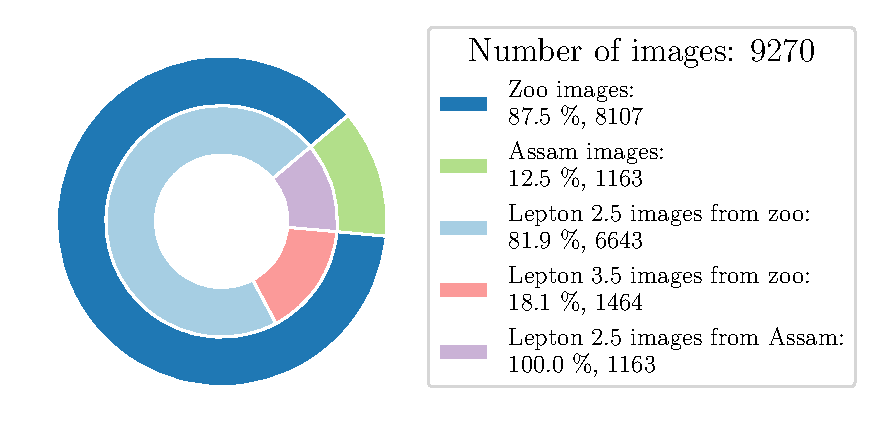
\includegraphics{nested_donut1.pdf} 
    \caption{Distribution of used images depending on image location and type of sensor.}
    \label{nested_donut1}
\end{figure}

    \item After manually inspecting the folder with goat images we saw that it mostly contained images of a goat herd, standing around a single elephant.
This folder was usable only for object localization ML models, where each goat could be tagged with a bounding box. 
In case of an image classification model, this sort of training data is not desirable, as it would be too similar to another separate class, in our case elephant class.
We therefore dropped goat images out of our training data entirely.

    \item We also realised that there was a large class imbalance, as seen on Figure \ref{nested_donut2} in favor to elephant class.
Number of elephant images was more than 4 times larger from the number of images of the all other classes combined.
This issue was solved with acquiring more images of the minority class, oversampling the minority class and additionally augmenting images in training phase.
\end{enumerate}

\begin{figure}[ht]
    \centering
    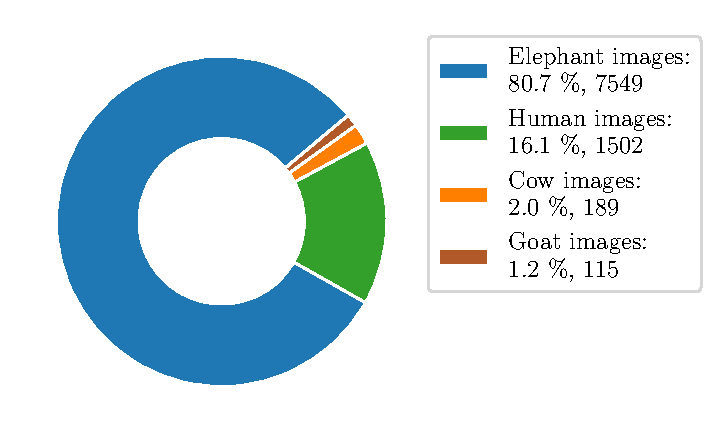
\includegraphics{nested_donut2.pdf} 
    \caption{Class distribution of thermal images.}
    \label{nested_donut2}
\end{figure}

\subsection{ Gathering thermal images}

As the amount of cow images was low compared to human and elephant classes and because we also did not had any images that would fit into nature/random class, we decided to gather them ourselves.
We wanted to do this as quickly and efficiently as possible so we build a prototype camera made out of FLIR Lepton 2.5 breakout board, Raspberry Pi Zero and power bank.
We used an open source library \cite{flir_github} for FLIR Lepton module which used a simple C program to take a single image with a thermal camera and save it to a Raspberry Pi.
Image of the setup can be seen on Figure \ref{cow_camera}.

\begin{figure}[ht]
    \centering
    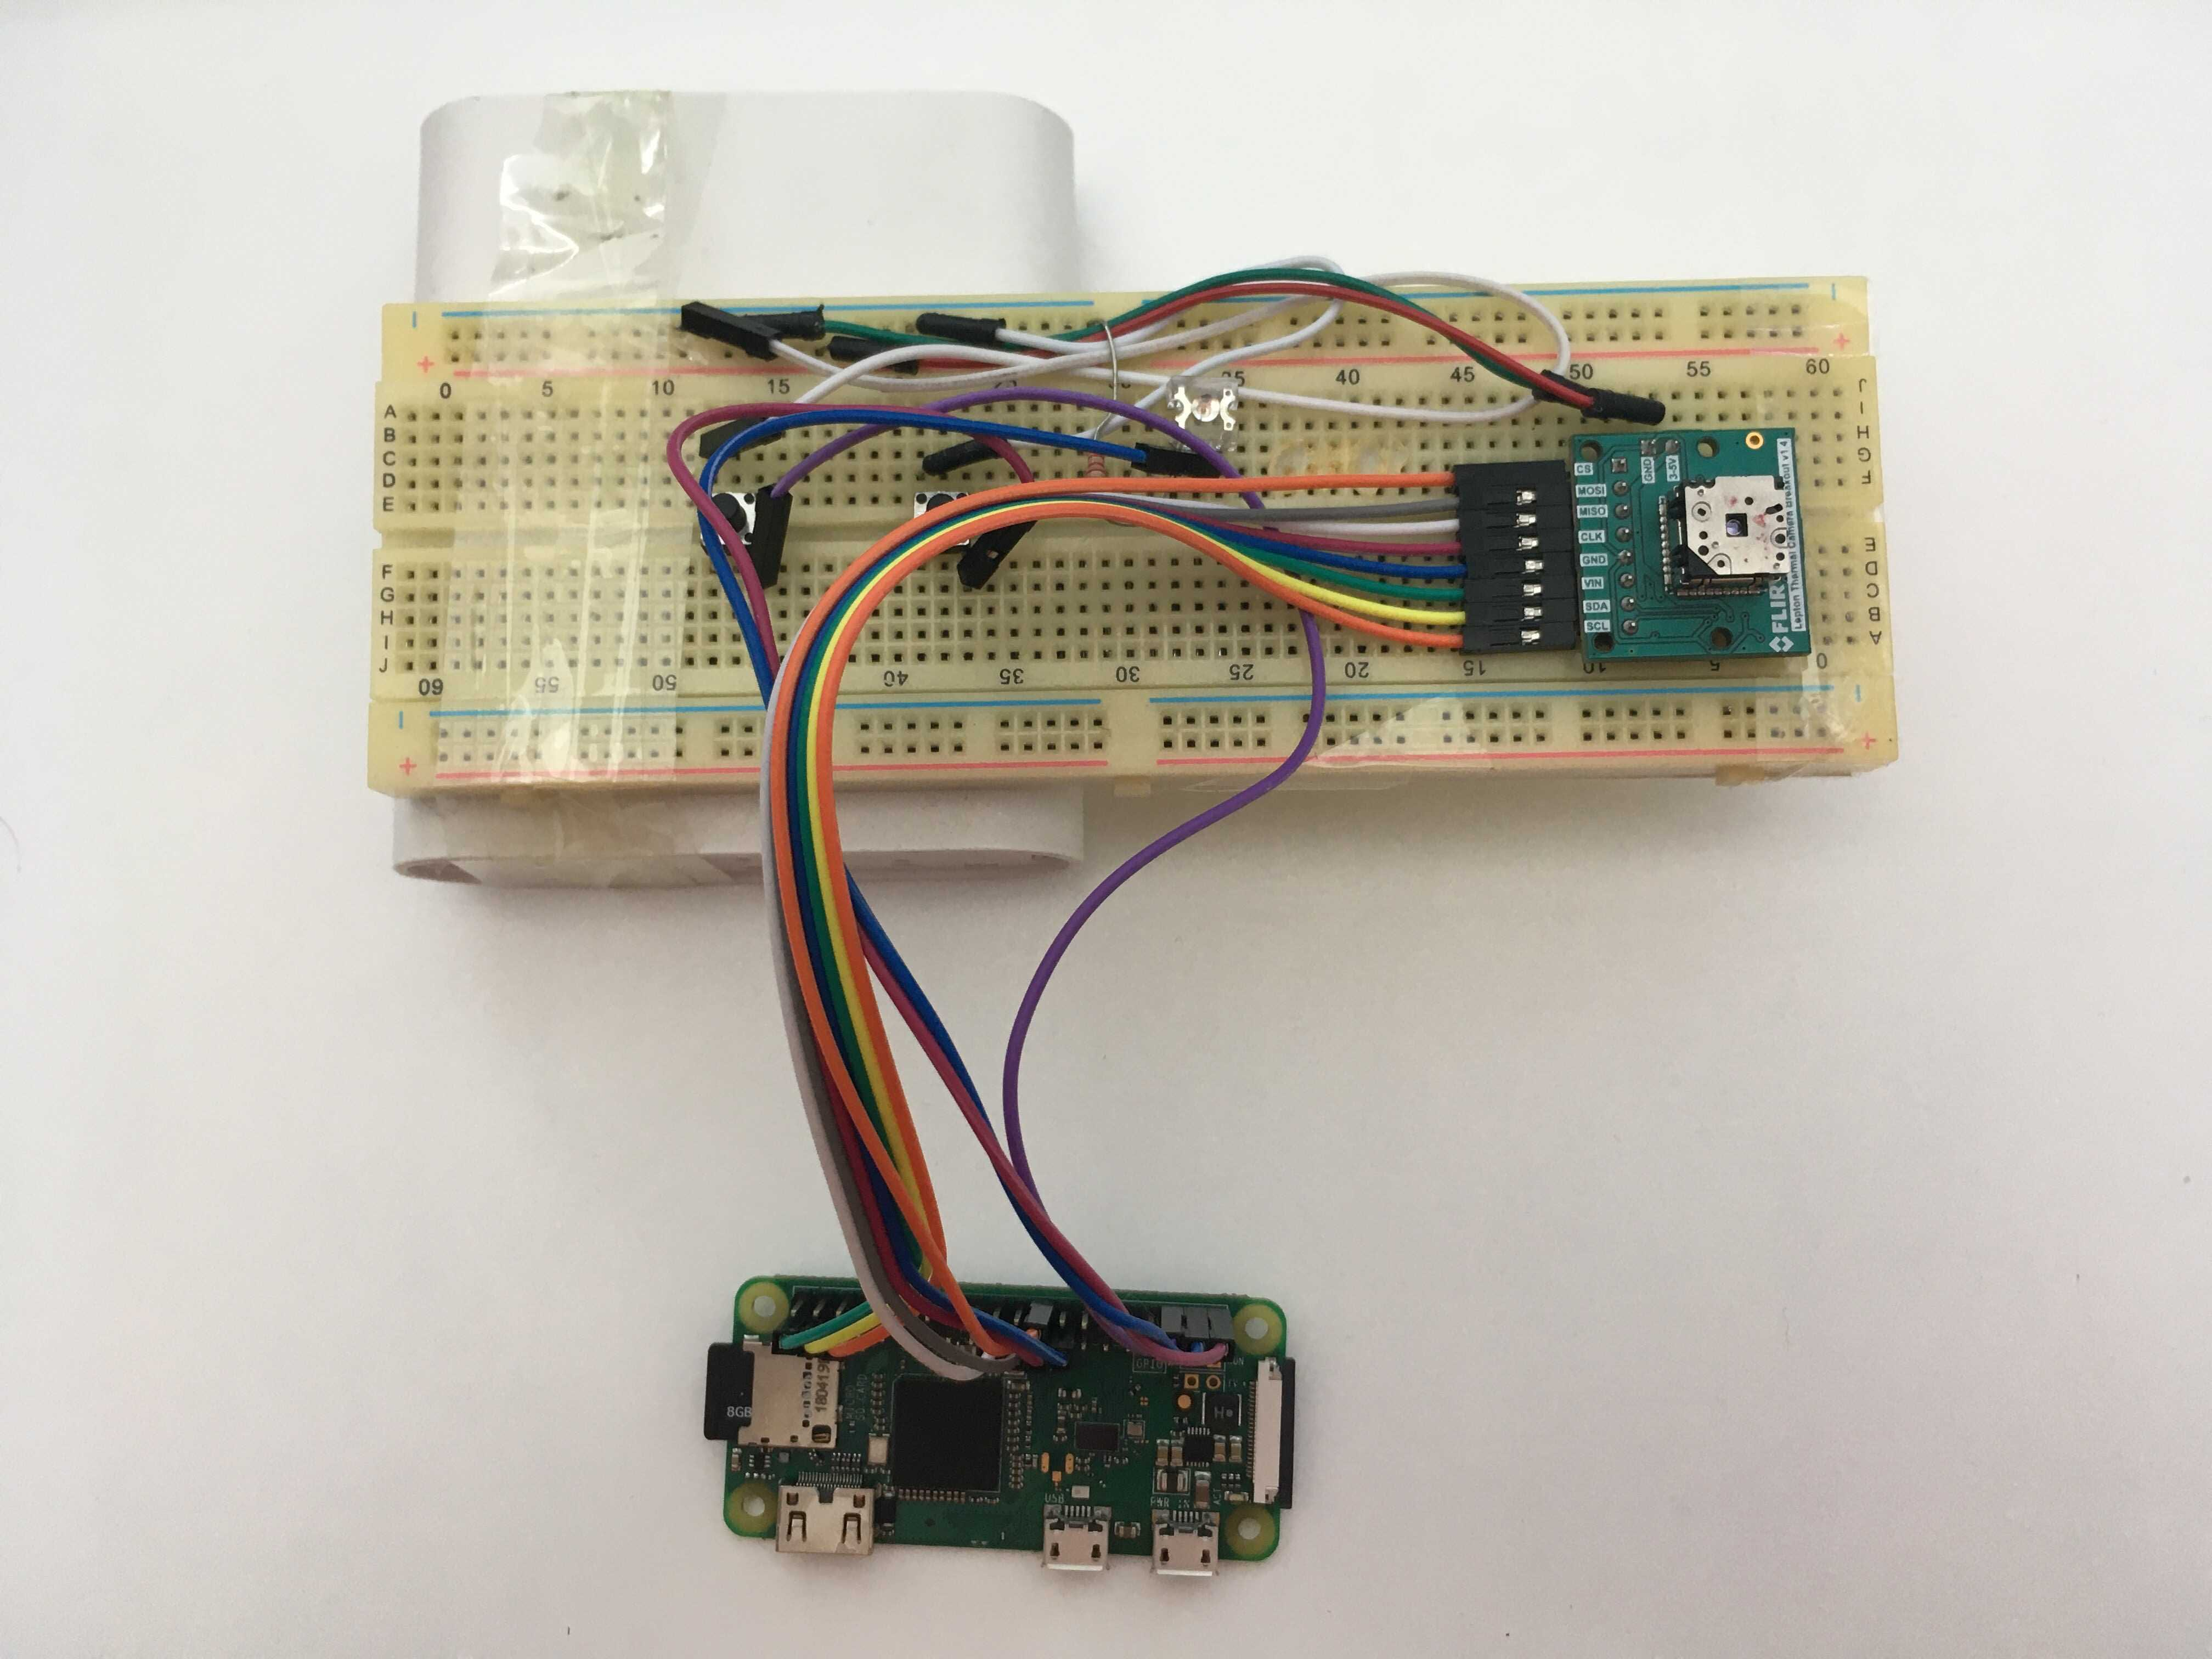
\includegraphics[width=1.0\linewidth]{cow_camera.jpg} 
    \caption{Camera setup used for taking thermal images with FLIR Lepton 2.5.}
    \label{cow_camera}
\end{figure}

We wrote a simple Python script which executed C program every time we pressed the trigger push-button.
Additional shutdown button was added to call the Raspberry Pi shutdown routine, as forcibly removing power from it would corrupt freshly taken thermal images on the Raspberry Pi's SD card.

With this setup we made 365 images of cows in varying conditions, 308 images of nature and 124 images of a human that were made on the go.
We then manually sorted images into appropriate folders and added them to the dataset.


\section{ Tools and development environment}

All of the work around image preparation and ML model creation was done in Python 3.6,
Numpy was used for image preprocessing, Pandas for Excel database manipulation and Matplotlib for plot generation.
Neural networks were designed in TensorFlow 2.4, using Keras high level API.

As training neural networks is a computationally demanding process, it would not be feasible to do it on a personal laptop.
We instead used Amazon's Elastic Compute Cloud web service.
Elastic Compute Cloud or EC2 enables users to create an instance of a server in a cloud with specified amount of processing power and memory.
Some instances come with dedicated software modules and dedicated graphics cards for extra boost in performance.
We created an instance of Linux server that came with TensorFlow, Numpy and other libraries pre-installed.
We interacted with the server's command line through SSH protocol.

Instead of writing Python scripts and executing them through command line, we used Juptyer Notebook. 
Juptyer Notebook is a web-based application that can run programs that are a mix of code, explanatory text and computer output.
Users can divide code into segments, which can be executed separately, visual output from modules such as Matplotlib is also supported.
To use Juptyer Notebook on our cloud instance, we had to install it and run it.
We could then access web service simply through web browser by writing the IP address of the server, followed by the default Juptyer Notebook server port, 8888.


\section{ Image preprocessing}

Image preparation phase is a pipeline process that differs from project to project.
Our process can be seen on Figure \ref{image_preparation}.

\begin{figure}[ht]
    \centering
    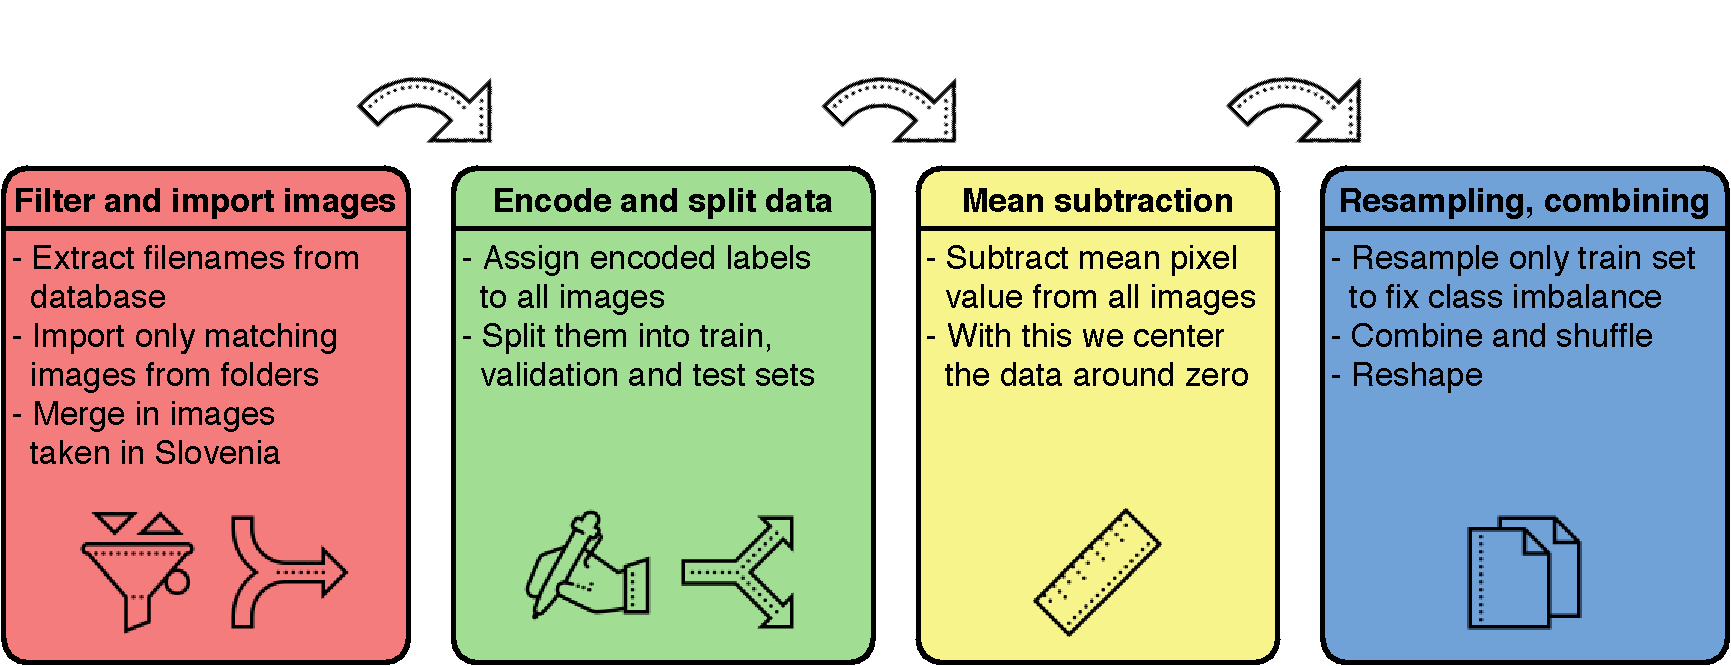
\includegraphics[width=1.0\linewidth]{image_preparation.pdf} 
    \caption{Image preparation pipeline that was used. Icons source: www.icons8.com.}
    \label{image_preparation}
\end{figure}

At the start of the process we compared filenames of each separate folder to the list of filenames found in Excel database.
We imported only the images found in both sources, as lists were not identical and we wanted to keep track of different metadata information.
As some images were made with two different FLIR Lepton cameras with different resolutions (60 x 80 and 120 x 160), we downscaled higher resolution images directly in the importing process.
After this we added images that were taken by us in Slovenia.
At this point we had four separate Numpy arrays, one for every class, with 3 dimensions: first dimension was a number of different images in that class, second and third dimensions stored image's pixel values (60 and 80 pixels respectively).

Next step was assigning labels to each image.
As the output of NNs are numbers, we can not just assign labels in strings format to data.
Instead we assigned every image a single number that represented that class, 0 for elephant, 1 for human, 2 for cow and 3 for nature/random class.
We shuffled images inside of each class and then split them into training, validation and test sets.

Training set is used for model training, while validation set helps to choose best model based on accuracy.
Test set is normally set aside and used only at the end, after the model is chosen, to asses how model performs on never seen data.
If we did not use validation set and only choose the best model according to test set, we would be overfitting a model and had no accurate measure how would our model perform on unseen data.

At end of this step we had 4 different Python dictionaries for each class.
Each dictionary had 3 key-value pairs for every training, validation and test set, which held image data and encoded labels.

We next applied simplest form of normalization to all images, a mean subtraction.
We calculated a two dimensional matrix that held mean values of pixels averaged over the whole training set, which we subtracted from all images, essentially zero centering the data.
This is a common preprocessing step in every ML image pipeline, which is usually combined with standardization\footnotemark.

\footnotetext{Standardization scales the whole range of input pixel values into -1 and 1 interval.
This is only needed if different input values have widely different ranges\cite{cs231n}.
Because images that were created with FLIR camera were all 8-bit encoded, therefore had same range, this was not needed.}

In the end we had to fix imbalance problem.
We achieved this by resampling the human, cow and nature/random classes.
Human class was resampled three times, while both cow and nature/random classes were resampled six times.
Figure \ref{resampled} shows distribution of training images before and after resampling.

\begin{figure}[ht] 
    \begin{subfigure}[b]{1\textwidth}
        \centering
        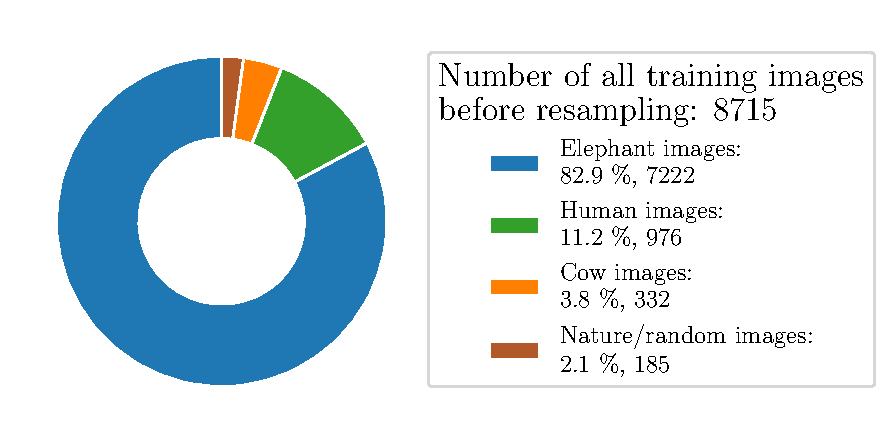
\includegraphics[width=1.0\linewidth]{nested_donut3.pdf} 
    \end{subfigure}
    \unskip\ \hrule\ 
    \begin{subfigure}[b]{1\textwidth}
        \centering
        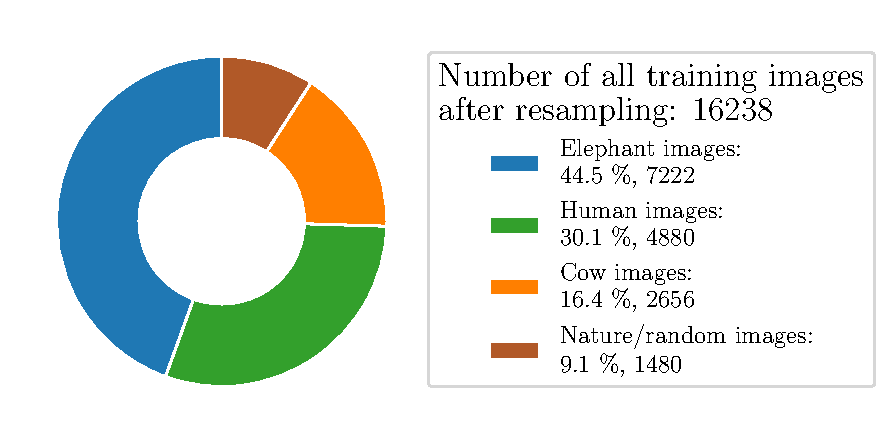
\includegraphics[width=1.0\linewidth]{nested_donut4.pdf} 
    \end{subfigure}
    
    \caption{ Distribution of training images before and after resampling.}
    \label{resampled}
\end{figure}

We only resampled training sets, not validation or test sets.
If we resampled everything, model would be seeing same image several times during testing, thus reporting incorrect accuracy in validation and test phase.

After resampling we merged and shuffled all data and reshaped it with Numpy from three dimensions to four, so it was ready for model training.


\section{ Model creation and training}\label{cnn_ref}

For creating CNN models we used Keras Sequential API and Keras Tuner model.
Sequential API abstracts a lot of low level details of model design.
When adding layers we are only specifying what type of layer we went, size of it and layer specific features. 
We do not need to keep track of any connections between or in layers, this is done automatically by Keras.

For a rough model architecture we decided to use a simplified version of a common CNN architecture that was shown in Figure \ref{convnet}.
The best way to present the model is by looking at the Sequential API code that created it, which is shown in Figure \ref{model_code}.

Model consists of two pairs of convolutional and max pooling layers, followed by a final convolutional layer.
Kernels are all the same size, 3 x 3, activations are set to ReLu function and padding is set to same, which means that a spatial dimension of a volume will not change in a convolutional layer.
The output volume of the last convolutional layer is flattened out into a single vector and fed into dense layer, which is followed by a dropout layer\footnotemark.

Last dense layer is a final output layer with only 4 neurons, each one representing one class.
Softmax activation is used to calculate class probabilities.

\footnotetext{ Dropout layer decides with probability $p$ in each training step how many activations from previous layer will be passed on to the next layer.
It is active only during training phase, during testing phase activations are multiplied with $(1-p)$ factor to compensate.
It is a very popular type of regularization technique which makes models more robust to the input data\cite{geron}.}

\definecolor{codegreen}{rgb}{0,0.6,0}
\definecolor{codegray}{rgb}{0.5,0.5,0.5}
\definecolor{codepurple}{rgb}{0.58,0,0.82}
\definecolor{backcolour}{rgb}{0.95,0.95,0.92}

\lstdefinestyle{mystyle}{
    backgroundcolor=\color{backcolour},   
    commentstyle=\color{codegreen},
    keywordstyle=\color{magenta},
    numberstyle=\tiny\color{codegray},
    stringstyle=\color{codepurple},
    basicstyle=\linespread{0.9}\ttfamily\footnotesize,
    breakatwhitespace=false,         
    breaklines=true,                 
    captionpos=b,                    
    keepspaces=true,                 
    numbers=left,                    
    numbersep=5pt,                  
    showspaces=false,                
    showstringspaces=false,
    showtabs=false,                  
    tabsize=2
}

\lstset{style=mystyle}

\begin{figure}[ht] 
    \begin{lstlisting}[language=Python]
        model = models.Sequential()

        model.add(Conv2D(filter_num_1, (3, 3), 
                         activation='relu', 
                         padding="same", 
                         input_shape=(60,80, 1)))

        model.add(MaxPooling2D((2, 2)))

        model.add(Conv2D(filter_num_2, (3, 3), 
                         activation='relu', 
                         padding="same")

        model.add(MaxPooling2D((2, 2)))

        model.add(Conv2D(filter_num_3, (3, 3), 
                         activation='relu', 
                         padding="same")

        model.add(Flatten())

        model.add(Dense(dense_size, activation='relu'))
        model.add(Dropout(dropout_rate))
        model.add(Dense(4), activation='softmax')
    \end{lstlisting}
    \caption{ Distribution of training images before and after resampling.}
    \label{model_code}
\end{figure}





\section{ Model optimization}

For model optimization phase we wrote a Python script that took model in .h5 format and converted it into four differently optimized tflite models:
\begin{itemize}
    \item \textbf{Non-quantized tflite model,} no quantization, just basic conversion from .h5 to .tflite format is done.
    \item \textbf{float16 model,} weights are quantized from 32-bit to 16-bit floating-point values. Model size is split in half and accuracy decrease is minimal, but there is no boost in execution speed.
    \item \textbf{dynamic model,} weights are quantized as 8-bit values, but operations are still done in a floating-point math. Models are 4 times smaller and execution speed is faster when compared to float16 optimization but slower from full integer optimization.
    \item \textbf{Full integer model,} weights, biases and math operations are quantized, execution speed is increased. It requires representative dataset at conversion time.
\end{itemize}

Full integer model is an ideal choice for running models on microcontrollers, however it should be noted that not all operations have full integer math implementations in TFLite Micro.

Created .tflite models had to be converted into a format that is understandable to a microcontroller.
This was done with the \textbf{xxd}, a Linux command line tool which creates a hex dump out of any input file.
As a input parameter we give xxd our .tflite model and set the -i flag.
Xxd tool will then create a hex dump of our model and format it as a char array in C programming language. 
We then created .c file with char array values and a .h file with its declaration, which we can later call from our application code.


\section{ Neural network model design in Edge Impulse Studio}
